%%%%%%%%%%%%%%%%%%%%%%%%%%%%%%%%%%%%%%%%%
% University/School Laboratory Report
% LaTeX Template
% Version 3.1 (25/3/14)
%
% This template has been downloaded from:
% http://www.LaTeXTemplates.com
%
% Original author:
% Linux and Unix Users Group at Virginia Tech Wiki 
% (https://vtluug.org/wiki/Example_LaTeX_chem_lab_report)
%
% License:
% CC BY-NC-SA 3.0 (http://creativecommons.org/licenses/by-nc-sa/3.0/)
%
%%%%%%%%%%%%%%%%%%%%%%%%%%%%%%%%%%%%%%%%%

%----------------------------------------------------------------------------------------
%	PACKAGES AND DOCUMENT CONFIGURATIONS
%----------------------------------------------------------------------------------------

\newcommand{\abs}[1]{\left| #1 \right|} % for absolute value
\newcommand{\avg}[1]{\left< #1 \right>} % for average

\renewcommand{\d}[2]{\frac{d #1}{d #2}} % for derivatives
\newcommand{\dd}[2]{\frac{d^2 #1}{d #2^2}} % for double derivatives
\newcommand{\pd}[2]{\frac{\partial #1}{\partial #2}} 
% for partial derivatives
\newcommand{\pdd}[2]{\frac{\partial^2 #1}{\partial #2^2}} 
% for double partial derivatives
\newcommand{\pdc}[3]{\left( \frac{\partial #1}{\partial #2}
 \right)_{#3}} % for thermodynamic partial derivatives
\newcommand{\ket}[1]{\left| #1 \right>} % for Dirac bras
\newcommand{\bra}[1]{\left< #1 \right|} % for Dirac kets
\newcommand{\braket}[2]{\left< #1 \vphantom{#2} \right|
 \left. #2 \vphantom{#1} \right>} % for Dirac brackets
\newcommand{\matrixel}[3]{\left< #1 \vphantom{#2#3} \right|
 #2 \left| #3 \vphantom{#1#2} \right>} % for Dirac matrix elements
\newcommand{\grad}[1]{\gv{\nabla} #1} % for gradient
\let\divsymb=\div % rename builtin command \div to \divsymb
\renewcommand{\div}[1]{\gv{\nabla} \cdot #1} % for divergence
\newcommand{\curl}[1]{\gv{\nabla} \times #1} % for curl

\documentclass{article}

\usepackage{graphicx} % Required for the inclusion of images
\usepackage{natbib} % Required to change bibliography style to APA
\usepackage{amsmath}
\usepackage{setspace}
\usepackage{amssymb}
\renewcommand{\labelenumi}{(\alph{enumi})}

\setlength\parindent{0pt} % Removes all indentation from paragraphs

\renewcommand{\labelenumi}{\alph{enumi}.} % Make numbering in the enumerate environment by letter rather than number (e.g. section 6)

%\usepackage{times} % Uncomment to use the Times New Roman font

%----------------------------------------------------------------------------------------
%	DOCUMENT INFORMATION
%----------------------------------------------------------------------------------------

\title{WiPAL Fabry-Perot\\ Spectrometer} % Title

\author{Ken \textsc{Flanagan} and Jason \textsc{Milhone}} % Author name

\date{\today} % Date for the report

\begin{document}

\maketitle % Insert the title, author and date


% If you wish to include an abstract, uncomment the lines below
% \begin{abstract}
% Abstract text
% \end{abstract}

%----------------------------------------------------------------------------------------
%	SECTION 1
%----------------------------------------------------------------------------------------

\section{Introduction}
Need to add a nice little introduction here about what we're doing etc...

%----------------------------------------------------------------------------------------
%	SECTION 2
%----------------------------------------------------------------------------------------

\section{Optical Layout}
\begin{figure}
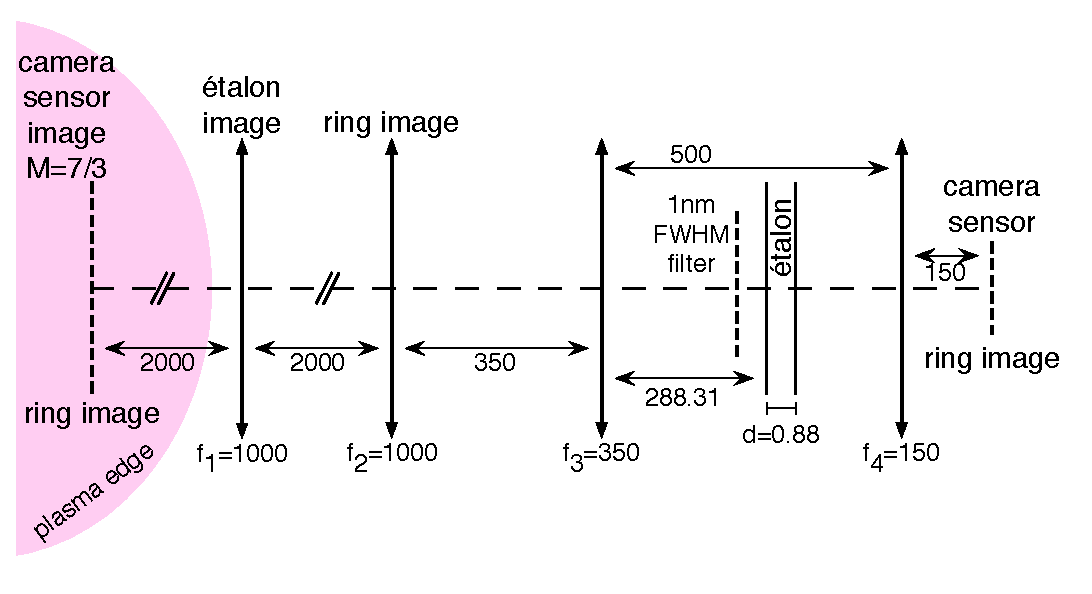
\includegraphics[width=\textwidth]{Images/FP_Optical_Schematic.eps}
\caption{Optical schematic of Fabry-P\'{e}rot spectrometer used on WiPAL. All lengths are in units of millimeters. \label{fig:opticalsetup}}
\end{figure}
The optical layout for the WiPAL Fabry-P\'{e}rot spectrometer is shown above in Fig.~\ref{fig:opticalsetup}. The main components of this setup are a pair of lenses ($f_{t1}$ and $f_{t2}$) that form a telescope to bring light from the center of plasma to the \'{e}talon, another telescope formed by lenses $f_{3}$ and $f_{4}$ that focuses light through the \'{e}talon, and the camera sensor. 

%----------------------------------------------------------------------------------------
%	SECTION 3
%----------------------------------------------------------------------------------------

\section{Basic Fabry-P\'{e}rot Theory}
A Fabry-P\'{e}rot interferometer consists of a set of highly-reflective, partially transmitting parallel plates, called an \'{e}talon. Light enters the \'{e}talon and is reflected many times back and forth creating an interference pattern. This pattern can be used to determine the wavelength of the incident light. 
\begin{figure}
\includegraphics[width=\textwidth]{Images/etalon.png}
\caption{An \'{e}talon showing incident, reflected and transmitted light.
\label{fig:etalon}}
\end{figure}
Fig.~\ref{fig:etalon} shows a simple schematic of an \'{e}talon. Light incident at some angle, $\theta$, reflects back and forth in the cavity and then exits at the same angle, $\theta$. On each pass through the cavity, the light picks up a phase shift of
\begin{equation}
\phi = 
\end{equation}
Lot's of filler here... lala, the transmission function:
\begin{equation}
\frac{I_{t}}{I_{i}} = \left[1+Q\sin{\pi m}^{2}\right]^{-1}
\label{eq:airy}
\end{equation}
Where
\begin{equation}
Q = \frac{4R}{(1-R)^{2}} = \frac{2}{\pi}\mathcal{F}^{2}
\end{equation}
Then this happens a bunch, blah blah then you get the glorious interference condition:
\begin{equation}
m\lambda = 2nd\cos{\theta}
\end{equation}
If we use a lens of focal length, $f$, the $\cos{\theta}$ term can be rewritten in terms of $f$ and the radius across the imaging plane, $r$. This gives us
\begin{equation}
m\lambda = 2d \frac{f}{\sqrt{f^{2}+r^{2}}}
\label{eq:inf_con}
\end{equation}
where we have absorbed $n$ into $d$, giving us an effective \'{e}talon spacing.

%----------------------------------------------------------------------------------------
%	SECTION 4
%----------------------------------------------------------------------------------------

\section{Fabry-P\'{e}rot Spectroscopy}
Given the interference condition (eq.~\ref{eq:inf_con}) and the Airy function output of the interferometer (eq.~\ref{eq:airy}), the output of the Fabry-P\'{e}rot for a given wavelength can be calculated. Looking at the interference condition, $m$ for a given $\lambda$ is given by 
\begin{equation}
m = 0,\,1,\,2\,...\,m_{0}\leq\frac{2d}{\lambda}
\end{equation}
where $m_{0}$ must be less than the $m$ given on the optical axis (when $\cos{\theta}=1$), $2d/\lambda$. Written another way,
\begin{equation}
m_{0} = \text{m of first interference peak} = \frac{2d}{\lambda} - \epsilon
\end{equation}
where $0\leq\epsilon<1$. Or, even simpler, $m_{0}=\text{Floor}[2d/\lambda]$. The interference condition is met by integer $m$, so this means that subsequent peaks will have $m_{j}=m_{0}-j$ for $j=0,\,1,\,2\,...$. (Note: $m$ decreases as we move away from the optical axis, because $\cos{\theta}$ decreases from $\theta=0$ to $\theta=\pi/2$.) In terms of the interference condition, this gives us:
\begin{equation}
m_{j}=m_{0}-j =\frac{2d}{\lambda}\frac{f}{\sqrt{f^{2}+r_{j}^{2}}}
\label{eq:mj}
\end{equation}
where $r_{j}$ is the radial location of peaks for that given wavelength. Inverting this equation to solve for peak locations gives,
\begin{equation}
r_{j} = f\sqrt{\left(\frac{2d/\lambda}{m_{0}-j}\right)^{2}-1}=f\sqrt{\left(\frac{2d/\lambda}{\text{Floor}[2d/\lambda]-j}\right)^{2}-1}
\end{equation}

All of the above calculation works for a given, single wavelength, but we are interested in what the Fabry-P\'{e}rot output for a given input spectrum, $B(\lambda)$, looks like. For this we need to integrate over all wavelengths. The output as a function of radius across the ccd will be:
\begin{equation}
I(r) = \int_{0}^{\infty} \frac{B(\lambda)\,d\lambda}{1+Q\sin^{2}{\left(\pi \frac{2d}{\lambda}\frac{f}{\sqrt{f^{2}+r^{2}}}\right)}}
\label{eq:pattern}
\end{equation}

\subsection{Mapping $r$ to $\lambda$}
In order to extract spectral information from the interference pattern given by eq.~\ref{eq:pattern}, a mapping must be made from $r$ to $\lambda$ space. This can be done by considering the change in $r$, $\Delta r$, for a given change in $\lambda$, $\Delta\lambda$. From eq.~\ref{eq:mj}, we see that if $\lambda\rightarrow\lambda+\Delta\lambda$, $r_{j}\rightarrow r_{j}+\Delta r$ in order to keep $m_{j}$ an integer. If we limit the change in $\lambda$ to less than a free spectral range, then
\begin{equation}
m_{0}=\text{Floor}\left[\frac{2d}{\lambda_{0}}\right]=\text{Floor}\left[\frac{2d}{\lambda_{0}+\Delta\lambda}\right]
\end{equation}
Under this condition we have a relation between $\Delta\lambda$ and $\Delta r$ given by
\begin{equation}
m_{0}-j = \frac{2d}{\lambda_{0}+\Delta\lambda}\frac{f}{\sqrt{f^{2}+(r_{j}-\Delta r)^{2}}}
\end{equation}
Solving for $\Delta r$, we get
\begin{equation}
\Delta r = r_{j} \pm f \sqrt{\left(\frac{2d}{(m_{0}-j)(\lambda_{0}+\Delta\lambda)}\right)^{2}-1}
\label{eq:dr1}
\end{equation}
This relation works quite well if you know $\lambda_{0}$, as is the case for a calibration lamp or a non-flowing plasma. However, if $\lambda_{0}$ isn't well known (only within a free spectral range-- which corresponds to a flow velocity of about 60 km/s for the Argon 488nm line), we can use eq.~\ref{eq:mj} to get $\lambda_{0}$ given $r_{j}$.
\begin{equation}
\lambda_{0}=\frac{2d}{m_{0}-j}\frac{f}{\sqrt{f^{2}+r_{j}^{2}}}
\label{eq:lam_sub}
\end{equation}
Now if we substitute this into eq.~\ref{eq:dr1}, we have
\begin{equation}
\Delta r = r_{j} \pm f\sqrt{\left(\frac{2d\sqrt{f^{2}+r_{j}^{2}}}{2df+\Delta\lambda(m_{0}-j)\sqrt{f^{2}+r_{j}^{2}}}\right)^{2}-1}
\label{eq:dr2}
\end{equation}
Now we need to satisfy our condition that we don't venture out of a free spectral range when doing this mapping. To start, we should figure out what $\Delta\lambda$ gives the same $r$ location for two consecutive orders. Because increasing $r$ means decreasing $\lambda$ and orders decrease as $r$ is decreased we have:
\begin{align}
m_{0}-j&=\frac{2d}{\lambda_{0}-\Delta\lambda}\frac{f}{\sqrt{f^{2}+r_{edge}^{2}}}\\
m_{0}-j-1&=\frac{2d}{\lambda_{0}+\Delta\lambda}\frac{f}{\sqrt{f^{2}+r_{edge}^{2}}}
\end{align}
solving for $r_{edge}$ in both these equations and setting the resulting expressions equal gives
\begin{equation}
\Delta\lambda_{FSR/2}=\frac{\lambda_{0}}{2(m_{0}-j)-1}=\frac{2d}{2(m_{0}-j)^{2}-(m_{0}-j)}\frac{f}{\sqrt{f^{2}+r_{j}^{2}}}
\end{equation}
where we have used eq.~\ref{eq:lam_sub} to substitute $\lambda_{0}$ with an expression using $r_{j}$. Now we can take this expression and plug it into eq.~\ref{eq:dr2} to get the range of $r$ for a given order. 




%----------------------------------------------------------------------------------------
%	BIBLIOGRAPHY
%----------------------------------------------------------------------------------------

%\bibliographystyle{apalike}

%\bibliography{sample}

%----------------------------------------------------------------------------------------


\end{document}